\subsection{Habitat Simulator and Lab- Overview}

We use the Habitat platform as a host for the EQA task. The name 'Habitat' is derived from  the notion of learning within and from an environment. Imitating our natural habitat, the Habitat platform facilitates spawning an agent in a simulated environments with the possibility of teaching the robot to preform different tasks. 

The perquisites needed to test or train an agent for a certain task in a given environment, are facilitated by a core component called  Habitat Simulator. Habitat Simulator is responsible for simulating an  environment and insinuating a robot in it. The simulator acts depending on the configurations given to it. 

The configurations are processed into commands in Habitat-lab before being passed to the simulator. Habitat lab is the second core component of the system. In addition to giving commands to the simulator, the Habitat Lab module acts as a pipeline that prepares the data-set of the corresponding task. The habitat-lab module,in other words, is the coordinator that informs the simulator of the required setting, and the data loader and processor that prepares the data for either training or testing. 

\begin{figure}[H]
\centering
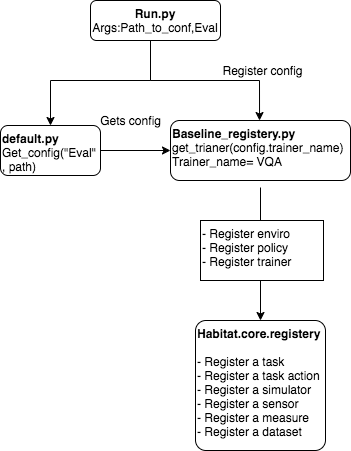
\includegraphics[scale=0.43]{images/configProcess.png}
\caption{Example of Habitat lab processing the configurations to implement validation for the VQA model }
\label{fig:configs}
\end{figure}

Figure \ref{fig:configs} resembles a map of the code structure when the habitat lab module is initiated to preform validation task for the VQA. Each task has its own configurations and in this example the task is 'VQA evaluation'. As seen in the figure \ref{fig:configs}, the module takes hierarchical steps in which each step is executed in accordance to the configuration of the given task. In the most down box of the structure we see parts of the commands directed for the simulator, such as insinuating an environment and sensors in the agent. Other commands include registering a data-set which takes part in lab module. 

\subsection{vision}

The vision of the system relies on egocentric 224x224 RGB images processed in CNN. The CNN encoding has the functionality of a “multi-task pixel-to-pixel prediction framework,” which consists of 4 {5x5 Conv, BatchNorm, ReLU, 2x2 Max-Pool blocks}, and they produce a fixed-size representation.“The range of depth values for every pixel lies in the range r0, 1s, and the segmentation is done over 191 classes”(p.11). (page,6). 

It  is possible to train the encoder-decoder on generating  three sensory information. The three decoders, which can also be referred to as sensors take the functionality of: 1) RGB reconstruction, 2) semantic segmentation, and 3) depth estimation. The latter sensors are used to obtain “object attributes (i.e., colors and textures), semantics (i.e., object categories), and environmental geometry (i.e., depth).” . 

In the baseline models, different tasks take different sensors.Not all the above-mentioned sensors are used in all the baseline tasks. Since navigation and VQA are trained and evaluated separately, we refer to them as separate "tasks". The two tasks in EQA take the following sensors: 

{Navigation}:  "depth" and "RGB". Depth sensor is essential for the agent's capability to navigate. With depth sensor it could estimate distances and avoid colliding with obstacles.  

{VQA}: The existent baseline VQA model uses the visual information with "RGB" data only. (No reason mentioned to why the other sensors are not used in the question-answering baseline module).  



%Hence- current hidden-state h_{t} and the current action are only %updated in the planner: 
%
%The controller executes the action  a_{t+1}. It takes then the 
%
%Hence, h_{t-1} and a_{t-1} carry no information at the 0 timestep %since no encoding or action been outputed by the planner at the 0 %step; Thus they are more like an initiation in this example.  
%
%The planner passes the current action a_{t} and the current hidden %state h_{t} to the controller 
%



\subsection{Data and Data-sets}

 Our method of generating questions is largely related to the structure of the data-sets in the initial EQA paper\cite{embodiedqa}. Understanding each part of the data-sets and their structure would give an insight into the work flow of generating questions to the task. In this section we elaborate on the source of the data-sets, their content, and our methods in processing the data. 
 

\subsubsection{Semantic annotations in Matterport}

%(restructuring is required-- more precision) (examples to rephrase-- why do we need the %location in global coordinates and why the camera views are also important)
\paragraph{Annotations}
In the Matter port annotations, Each house environment comes with three files. The three files are x.house,x.ply and x.. We collect the annotations from the x.house files house. 

Each house file comes with eleven line-types of annotations.\footnotetext{https://github.com/niessner/Matterport/blob/master/data\_organization.md}. The lines are marked by a capital letter as a marker; the first letter-marking to the last letter are as in this list [H,L,R,P,S,V,P,I,C,O,V]. Each letter-marker symbolizes a certain type of information. In this section, I am going to explain only the type of information that we use in this project.

The only data we extract from the house file, is the "O". The "O" lines contain information about the objects in the house. Every line that begin with an O letter consist of one object in the house with a corresponding information about its geometry and location within a room and level-floor. Each "O" line looks as such: [ O object\_index region\_index category\_index px py pz  a0x a0y a0z  a1x a1y a1z  r0 r1 r2 0 0 0 0 0 0 0 0 ] 

The data of the object in the line seen above comes in a string form, and each section in the string represents different types of information. \textit{Object\_index}, the index of an object is what we refer to as the object ID. \textit{region index} is the room ID. \textit{category\_index} is the object's index in category map; this index is used to obtain the object's name from the category map.\textit{px py pz} represent the center of the box in (x,y,z) axis. \textit{a0x a0y a0z  a1x a1y a1z} these are the rotation of the OOBB and AABB. \textit{r0 r1 r2} represent the radius of the object from the center on the (x,y,z). Finally the last "0"s in the line have no meaningful value, and therefore are ignored. 

\paragraph{Views of the geometric data}

 The geometric information consist of elements as location of an object, region or level, defined by their center in a world coordinate system, as seen in the previouse section. Other information is the size of the entity given its radius from its starting location (center).   

The camera views of the scenes are globally oriented \cite{Matterport3D}(p3). A way to allocate an object is to find its location in a accordance to global coordinates. Let's say the global coordinates start from the center of a house where the center of the house is (0,0,0) on the (x,y,z); and let's say all the objects are spawned through out the house's (x,y,z) axis where each objects location is defined by its distance to the house center. When annotated, the objects are viewed through a camera. The description of their geometric location, thus, should consider the view-postion of the camera. 

\begin{figure}[H]
\centering
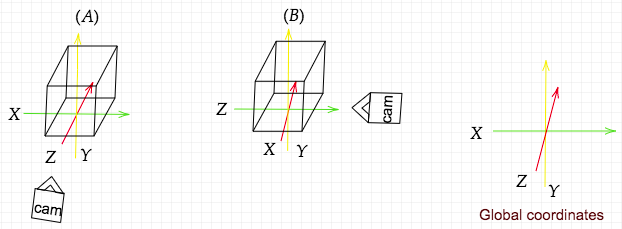
\includegraphics[scale=0.53]{images/campos.png}
\caption{The camera in graph A views the objects from global perspective(readers perspective). The view of the camera in graph B is rotated. The rotation is resembled in the the axis's representation }
\label{fig:campos}
\end{figure}

In graph (A) in \ref{fig:campos}, we see that the camera-view of coordinates align with the global coordinates.The (x,y,z) that go through each object in graph(A) and graph (B) are the view of the axis in reference to the camera. However, if the camera is positioned to the right of the object from our view, as in graph (B), then we say that the camera view of coordinates is not aligned with the global view. We notice in graph (B) that from the camera view, the "global X" is "Y" and vice versa.

Some geometric calculations cannot be preformed if the location measurements are not relative to each other. For example, if we want to calculate the distance between objects the locations must be consistent with one reference point. The camera position is changing and if the location of an object is referenced by the camera's position then we would get locations relative to the changing position of the camera in a time-span. 

To globalize the orientation of the view, measures such as top-down view of a map, or calculating the rotation of the camera from the global center. While the global locations are crucial for measuring the distance, other point-views are also crucial for other purposes. There are three essential coordinate systems to know when working in a 3D environments: 

\textbf{1. World coordinates}(global):  World coordinates(global): The coordinate system that starts at the center of the world; a house in our example. The center of an object in this coordinate system, is then decided by its distance to the center of the world. 

\textbf{camera-view coordinates:} The coordinates from the camera's views. The center of this coordinate system is the position of the camera. The center of the object in this world is defined by its distance to the camera. 

\textbf{3. Local view:} The center of the local view is the object itself. 

The center of all these views is (0,0,0). We described above that the world coordinate system allows us to measure distance between objects in a world map. The camera view is useful if a robot is expected to navigate an environment and describe spatial relations between objects such as "next to", "above". The local view could tell about the size of an object. In particular, the (x,y,z) from a local point of view tell about how far the object stretches from its center where the center is (0,0,0). The local view can be referred to as "radius". 

MatterPort 3D provide the views decribed above. We discuss in more detailed the usage of the object's location in global coordinates and the local view in details in the implementation part.  

\paragraph{Processing geometric data}

\begin{figure}[H]
\centering
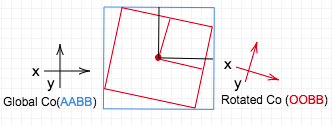
\includegraphics[scale=0.5]{images/A-OB.png}
\caption{2D AABB represented in blue square with its axis aligning with the world view of axis. 2D OOBB represented in red square has its axis rotated from the global view }
\label{fig:A-OB}
\end{figure}


The geometric information can be classified into two main categories. In a 3D environment we can imagine each object having  a labelling box rotated and oriented around its shape, and other box that bounds the first box with the global coordinates. In figure \ref{A-OB} we see a demonstration of the two boxes in 2d squares. The red box, that is meant to surround an object, is referred to as 'Object Oriented Bounding Box' (OOBB). The coordinates of the OOBB are rotated with rotation of the object (rotated in accordance to the local view). The blue box is referred to as 'Axis Aligned Bounding box'(AABB). The axis of AABB are aligned with global coordinates. 

We extract and save one specific information type of each box. The feature we take is the "radii", or else can be referred to as half-extents. The half-extents (radius) can be helpful in representing the object in different ways.  

We use the radius of the OOBB box to calculate the size of an object. The volume of OOBB gives more precise estimation of the size of the object, as the box is more enclosed around the object.

We use the radius of AABB box to measure the distance of an object to other objects. We can measure the distance between objects in an environment by the distance between their centers. More precise measurements would be to measure the edges or the corners of the object. We get the corners by measuring how far the box stretches(given by radius) from the center.  

Important to mention that we locate entities on a map with coordinate points that are positioned in accordance to one coordinate system (grounded in a the global map). Otherwise the numbers that represent positions would be in-indicative of points in the global view . It is for the latter reasons, the centers (located globally) are helpful to measuring distance-- because they are located on the same coordinate basis.  

The AABB box, provide a straightforward estimation of the positions of the object's shape in the global map. The local view of the AABBs are aligned with world coordinates, therefore allocating its corners globally would only require an estimation of how its radius(given in alliance with world coordinates) stretches from the center.

True that the OOBB corners are better representatives of the objects corners, however, locating the oobb corners in the world map is not simply done by measuring how its radius stretches from the center in the direction of  the global axis as in AABB. The radius of the OOBB is given along its local view axis(its rotation), meanwhile the center point is given in the world axis. Thus, locating the positions of the OOBB, using the same radius-length measure, would require adjusting the radius to the direction of its rotation. Therefore, the global-alignment characteristic of the aabb provides a direct way to locating its edges.  


The corners of the OOBB would be the most precise representation of the corners of an object. 



\subsubsection{EQA (Task Dataset)}

Our method for generating questions relies on imitating the structure of teh EQA-mp3d data-set. In this section we give a review of the EQA-mp3d structure and attributes.   

\paragraph{Structure}

\begin{figure}[H]
\centering
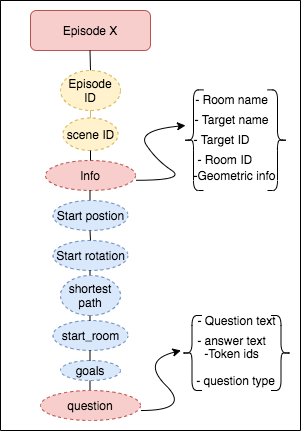
\includegraphics[scale=0.5]{images/episode1.png}
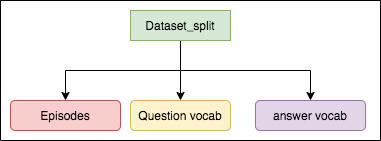
\includegraphics[scale=0.5]{images/datasplit1.png}
\label{fig:episode}
\caption{}
\end{figure}

In figure \ref{fig:episode} we see the top structure of the val and test. \textit{Episodes} refer to each question-function in the data-set split. \textit{Question vocab} and \textit{answer vocab} contain the same elements as dictionary keys. The elements are: [word list,stoi,itos,num vocab,pad token].

"Question vocab" and "answer vocab" in the "train" and "val" are identical to each other. When using each split of the dataset, the answer-tokens that are considered are the ones contained within the episodes instead of the word-lists mentioned above. 

Each question-sample is an episode that consist of multiple layer information. The structure of one episode of all the "episodes" is as seen in figure(x). We describe the elements of an episode in the following:  

\textbf{House ID}: The house ID given by the house ids in MatterPort3D.
\textbf{Episode ID}: The episode index in the range of the split's length. \hspace{1.5cm}
\textbf{Info}: This element contains all the information about the the object and room in a question. The information is structured as such: 

Information about the traget-object is the first layer within "info": 

\textit{centroid}: The center of the object's box in the global coordinates. Box is the area that labels  the object. When the center is globally oriented we would refer to this center and box as Axis-aligned bounding box(AABB), which means that (x,y,z) axis of the center are aligned with global coordinates. 

\textit{radi}: It tells how far the box (object) stretches from its center one direction of each axis. The value of radii is relative to the object itself (from the local view), where the center is zero. If we have, for example a radi of (2,1,4), this means that the object's box stretches +2 and -2 from the center on the x axis. The boundaries of the object's box relative to itself is referred to as object oriented bounding box (OOB). 

\textit{level}: at which level-floor of the house  is the object located in. 

\textit{room-id}, \textit{room name},\textit{obj Id},\textit{room name} : Room ID, room name and object ID as given by semantic annotation in  Matterport3D. Many of the objects are re-named, mostly names in hyponymes changed to hypernym category such as: round-sofa, l-shaped sofa changed to their hypernym category "sofa". 

The second layer is information about the room: 

Information about the room is similar to the type of information given for the objects. Th information is \textit{floor-level}, \textit{room-id}, \textit{room name},

Final layer consist of a "question-meta" which includes the color of the object. This section also includes question-entropy ..... 

The elements that are marked in blue in figure(x) are navigation-related material. 

\textbf{start position}: The start positions are all unique. For each unique question in the data set there is fifteen different starting position. 

\textbf{rotations}: This is the rotations that the agent have to do while navigating. It stands as supplementary information for the shortest path 

\textbf{goals}: Goals are the destinations that the agent should reach in navigation. The goals stand for the possible view points from where the the target object can be looked at by the robot. Each view point consist of geometric position and the rotation toward the target object respective to the position. 

%\begin{figure}
%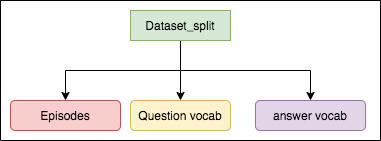
\includegraphics[scale=0.5]{images/datasplit1.png}
%\end{figure}







